\section{Rappel des fonctionnalités de la solution informatique et organisationnelle}

La solution spécifique est une solution développée spécialement pour l’entreprise. Elle ne repose pas en tout ou partie, contrairement à la solution standard, sur un progiciel déjà existant face auquel elle devra adapter ses processus. Ici, c’est la solution qui s’adapte à l’entreprise. \\

L’intégralité du logiciel doit donc être réalisé via des développements spécifiques, ainsi que les développements évolutifs ultérieurs à la mise en place de la solution. Il faut donc prévoir une équipe pour réaliser ce développement, qu’il soit interne ou sous traité.

\section{Chiffrages des coûts (d'acquisition et de possession)}

\begin{shaded}
\noindent\textsc{Note :}

    Voir Annexe B pour le tableau d'évaluation.
\end{shaded}

La mise en place d’une solution spécifique nécessite des investissements initiaux conséquents, qui correspondent en majeur partie à des immobilisations corporelles, basées sur du matériel informatique, à des immobilisations incorporelles, basées sur des licences logicielles et à des coûts de développement qui interviennent lors du déploiement du projet. L’important nombre de coûts d’acquisition découle sur un montant fort important d’investissement.

Les coûts de possession associés à la solution spécifique sont également fort important, les coûts de maintenance étant notamment élevés, ces derniers correspondant à 12\% des investissements initiaux. Les charges salariales correspondant aux nouveaux postes en charge de la gestion des nouveaux éléments du système d’information correspondent également à une augmentation de ces coûts de possession.

\begin{figure}[H]
    \noindent\makebox[\textwidth]{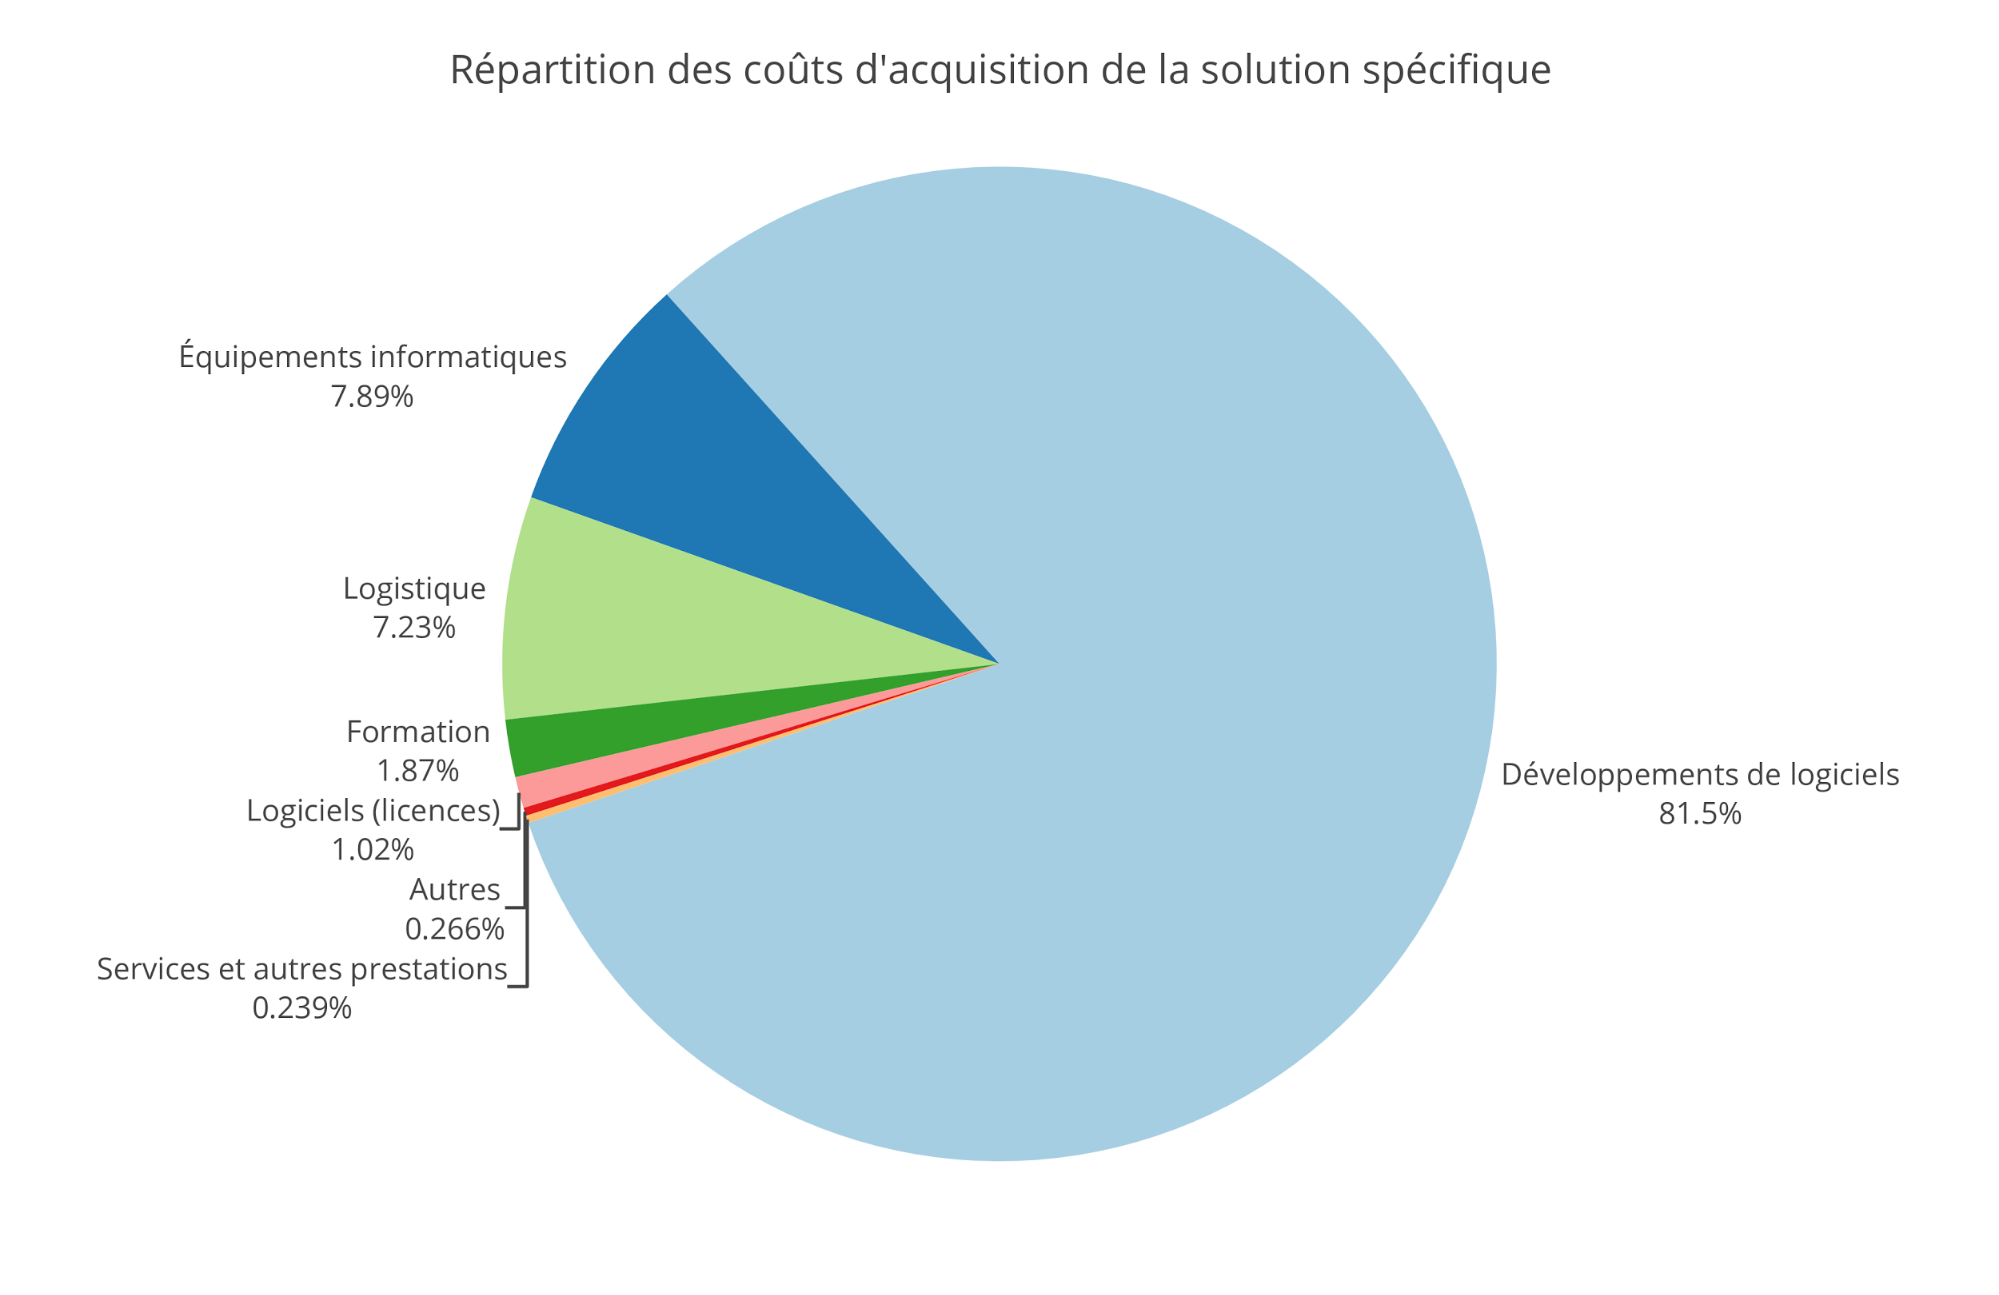
\includegraphics[width=12cm]{figures/cout_acquisition_sol_specifique.png}}
\end{figure}

\begin{figure}[H]
    \noindent\makebox[\textwidth]{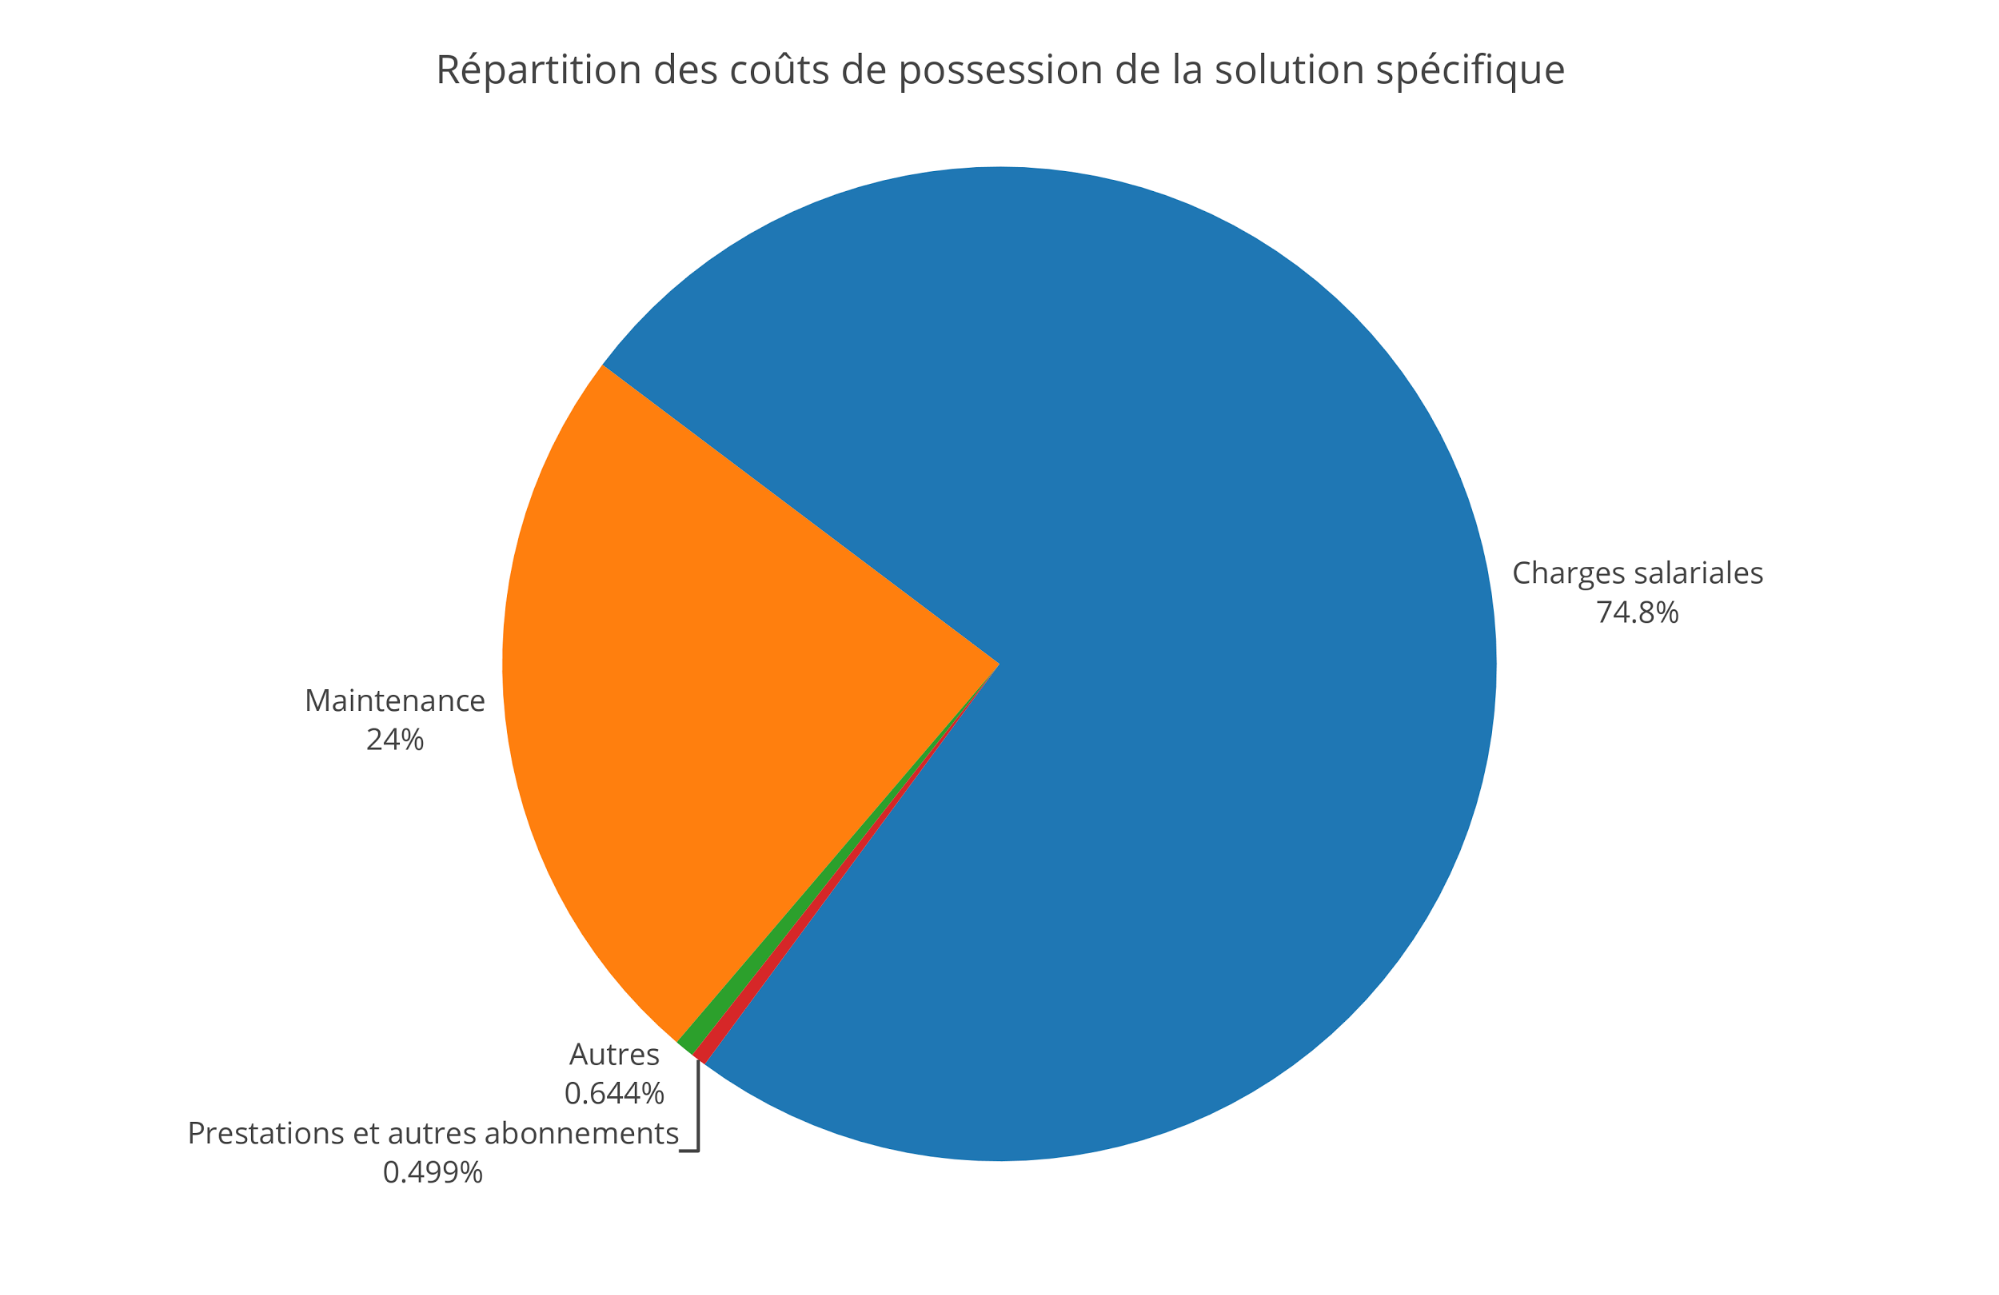
\includegraphics[width=12cm]{figures/cout_possession_sol_specifique.png}}
\end{figure}

\section{Retour sur investissement (gains)}

\begin{shaded}
\noindent\textsc{Note :}

    Voir Annexe B pour le tableau d'évaluation.
\end{shaded}

Le retour sur investissement de la solution spécifique est plus important, celui-ci s’élevant à 594 762,13 euros par an. En effet, la mise en place d’une solution sur mesure aux besoins de SPIE Sud-Est favorise grandement l’amélioration de la productivité de ses acteurs, sans pour autant bouleverser leurs habitudes de travail. Ainsi, la productivité des employés est augmentée, et les indicateurs mis en place permettent de réduire les risques tout en augmentant les performances réalisées par l’entreprise, expliquant ainsi le bon niveau de gain annuel, lié aux investissements réalisés en amont. \\

Cependant, étant donné l’importance des investissements ayant du être réalisés afin de mettre en oeuvre cette solution spécifique, celle-ci présente un délai de retour sur investissement de 24 mois, qui est plus long que celui proposé par la mise en place de la solution standard, avec toutefois un meilleur taux de retour sur investissement sur le long terme.

\section{Évaluation des autres critères de comparaison}

La solution est plus facile à faire évoluer et permet des développements spécifiques pour améliorer ou faire évoluer la solution. \\

A priori, elle permettra de ne pas trop modifier la structure du SI de l’entreprise. Ensuite, elle premettra de ne pas trop déstabiliser les collaborateurs de SPIE en offrant une interface qui sera plus cohérente avec le reste de leurs applications. \\

La sécurité de l’application sera dépendante de la sécurité générale des serveurs de SPIE, nous ne pouvons pas nous prononcer donc trop sur ce point. En revanche la fiabilité sera peut être moins bien car elle sera basée sur les anciens processus de SPIE, parfois peut adaptées. \\

L’évolution sera beaucoup plus simple que dans le cas de SAP étant donnée qu’elle sera interne à SPIE.